\documentclass{article}
\usepackage[utf8]{inputenc}
\usepackage{ctex}
\usepackage{amsmath}
\usepackage{float}
\usepackage{natbib}
% \usepackage{csvsimple}
\usepackage{tabularx}
\usepackage{booktabs}
\usepackage{longtable}
\usepackage{graphicx}
\graphicspath{{E:/Github/CourseWork/StochasticProcess/figs/}}


\title{随机过程大作业}
\author{张栩萌 \ 519070910031}
\date{May 2022}



\begin{document}

\maketitle

\section{实验目的}
1. 通过计算机模拟布朗运动,观察布朗运动的特性

2. 通过计算机模拟随机微分方程解的轨道,探究不同参数对轨道的影响,计算机模拟$X_1$的期望和方差

3. 熟练Python编程建模操作




\section{问题一:布朗运动}
布朗运动的定义为:若一个随机过程$\{X(t), t \ge 0\}$满足\\
1. $X(t)$ 是独立增量过程;\\
2. $\forall s, t>0, X(s+t)-X(s) \sim N\left(0, c^{2} t\right)$,即 $X(t+s)-X(s)$ 是数学期望为 0 ,方差为 $c^{2} t$ 的正态分;\\
3. $X(t)$ 关于 $t$ 是连续函数;\\
则称 $\{X(t), t \ge 0\}$ 是布朗运动或维纳过程。当 $c=1$ 时, 称 $\{X(t), t \ge 0\}$ 是标准布朗运动。

图\ref{fig:brown1}为在$[0, 1]$区间生成100个等距点,以0.1为时间间隔生成的标准布朗运动,图\ref{fig:brown1_10}为同样的区间节点下生成的$c=10$时的布朗运动。

\begin{figure}[H]
    \centering
    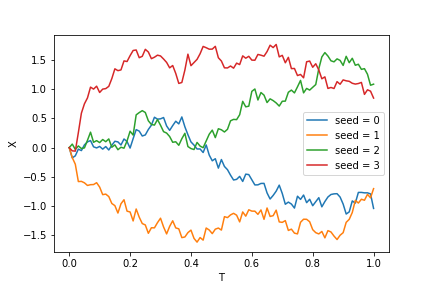
\includegraphics[scale=.6]{多条布朗运动轨道.png}
    \caption{多条标准布朗运动轨道}
    \label{fig:brown1}
    \end{figure}

\begin{figure}[H]
    \centering
    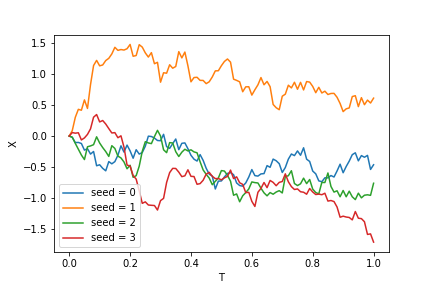
\includegraphics[scale=.6]{多条布朗运动轨道c=10.png}
    \caption{当$c=10$时多条布朗运动轨道}
    \label{fig:brown1_10}
    \end{figure}

因为参数$c$影响布朗运动的增量正态分布的方差,所以我们看到当$c=10$时布朗运动振荡的幅度明显大于标准布朗运动。




\section{问题二:股票价值随机微分方程}
设 $B=\left\{B_{t} ; t \geq 0\right\}$ 为标准布朗运动, $X=\left\{X_{t} ; t \geq 0\right\}$ 为如下随机微分方程的解:
$$
\left\{\begin{array}{l}
d X_{t}=\alpha\left(v-X_{t}\right) d t+\sigma d B_{t} \\
X_{0}=x_{0}
\end{array}\right.
$$
其中 $\alpha, v, \sigma, x_{0}$ 为常数。


我们采用不同的随机种子生成了随机微分方程解的多条轨道。

\begin{figure}[H]
    \centering
    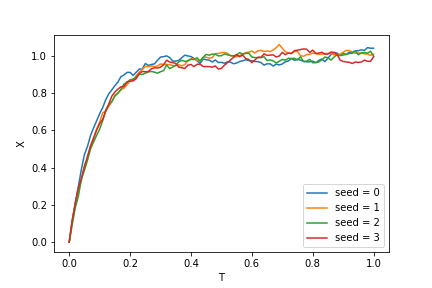
\includegraphics[scale=.6]{随机微分方程1的解多条轨道.png}
    \caption{随机微分方程1的解多条轨道}
    \label{fig:SDE1}
    \end{figure}







接下来我们测试不同参数对轨道的作用。

在微分方程中,$d B_t$ 是一个正态的扰动,前面的方程 $d X_{t}=\alpha\left(v-X_{t}\right) d t$ 表示了如果 $X_t$ 不等于 $v$ 的话,$X_t$ 会以一定速度向 $v$ 收敛。如果把 $X_t$ 看作是函数的话这个微分方程的函数解是 $f = \frac{1}{\alpha} exp{-\alpha t} + v + C$ 所以$v$代表了$X_t$的稳态。而$\alpha$就代表了收敛的速度。下面的实验对这些分析进行了验证


\begin{figure}[H]
    \centering
    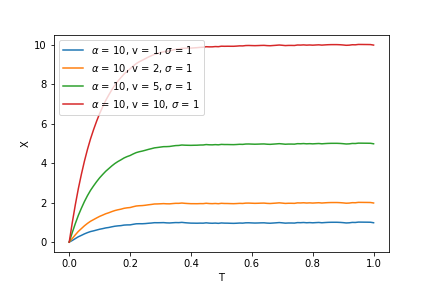
\includegraphics[scale=.6]{随机微分方程解1参数v.png}
    \caption{参数 $v$ 对随机微分方程1解的轨道影响}
    \label{fig:SDE1_v}
    \end{figure}



\begin{figure}[H]
    \centering
    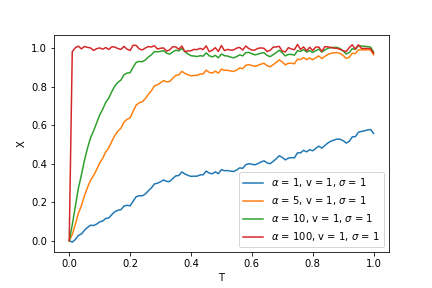
\includegraphics[scale=.6]{随机微分方程解1参数alpha.png}
    \caption{参数 $\alpha$ 对随机微分方程1解的轨道影响}
    \label{fig:SDE1_alpha}
    \end{figure}





\begin{figure}[H]
    \centering
    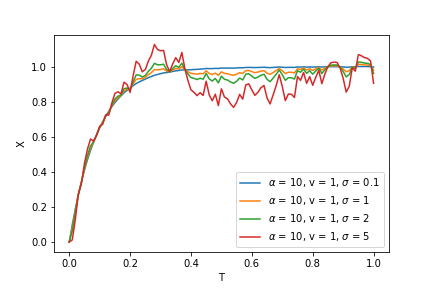
\includegraphics[scale=.6]{随机微分方程解1参数sigma.png}
    \caption{参数 $\sigma$ 对随机微分方程1解的轨道影响}
    \label{fig:SDE1_sigma}
    \end{figure}


\begin{figure}[H]
    \centering
    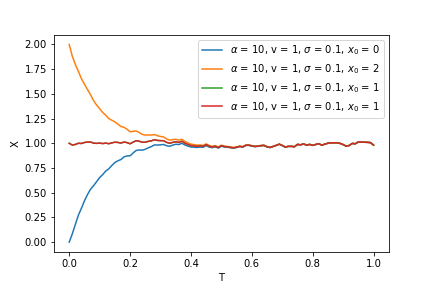
\includegraphics[scale=.6]{随机微分方程解1参数x0.png}
    \caption{参数 $x_0$ 对随机微分方程1解的轨道影响}
    \label{fig:SDE1_x0}
    \end{figure}


图\ref{fig:SDE1_alpha}说明$\alpha$ 越大收敛的速度越快;图\ref{fig:SDE1_sigma}说明$\sigma$ 越大噪声的振荡越大;图\ref{fig:SDE1_alpha}和图\ref{fig:SDE1_alpha}说明$v$ 决定$X_t$最终的稳态,而$x_0$决定$X_t$的初态。我们看到正如我们预期的一样,当$\sigma=0, v = x_0$的时候,初态就是稳态,且没有噪声,轨道是一条直线。

事实上,我们利用伊藤积分可以计算出这个随机微分方程的解,我们可以用解析解与前面我们数值计算的结果作为对照。

$$
\begin{array}{l}
EX_1 = v + (x_0 - v)e^{-\alpha} \\
DX_1 = \sigma^2 e^{-2\alpha} E((\int_0^1 e dB_u)^2) = \frac{\sigma^2}{2\alpha}(1-e^{-2a})
\end{array}
$$

我们看到前面数值实验得到的参数的作用与解析解显示的相同,接下来我们估计稳态分布的期望与方差,看看是否与上面的结论一致。

我们现在用Monte-Carlo模拟查看不同参数下$X_t$稳态分布的期望与方差。下面的实验都是在控制单一变量的条件下进行的,控制的变量默认为 $\alpha = 10, \ v=1,\ \sigma=0.1 , \ x_0 = 0$。

\begin{table}[H]
    \centering
    \caption{不同参数下的 $E(X_1)$ 和 $D(X_1)$}
    \begin{tabular}{l|l|l|l|l|l}
    \hline
    $\alpha$ & $E(X_1)$ & $D(X_1)$ & $v$    & $E(X_1)$ & $D(X_1)$ \\ \hline
    1     & 0.636873 & 0.004301 & 1    & 1.000939  & 0.000513 \\
    5     & 0.995510 & 0.000966 & 2    & 2.000912  & 0.000513 \\
    10     & 1.000939  & 0.000513 & 5    & 5.000832  & 0.000513 \\
    100    & 0.999987 & 0.000101 & 10   & 10.000699 & 0.000513 \\ \hline 
    $\sigma$ & $E(X_1)$ & $D(X_1)$ & $x_0$ & $E(X_1)$ & $D(X_1)$ \\ \hline
    0.01   & 1.00007  & 5e-06    & 0    & 1.000939  & 0.000513 \\
    0.1   & 1.000939 & 0.000513 & 2    & 1.000992  & 0.000513 \\
    0.2   & 1.001904 & 0.00205  & 5    & 1.001071  & 0.000513 \\
    0.5   & 1.004799 & 0.012815 & 10   & 1.001204  & 0.000513 \\ \hline
    \end{tabular}
\end{table}


    
实验结果表明,$v$与$E(X_1)$正比,$\sigma$的平方与$D(X_1)$正比,$\alpha$和$x_0$与这两个量无关。




\section{问题三:股票价值与价格随机微分方程}
设 $B=\left\{B_{t} ; t \geq 0\right\}$ 与 $W=\left\{W_{t} ; t \geq 0\right\}$ 为标准布朗运动, $X=\left(X_{t} , S_t\right)$ 为如下随机微分方程的解:
$$
\left\{\begin{array}{l}
d X_{t}=\alpha\left(v-X_{t}\right) d t+\sigma d B_{t} \\
d S_{t} = \theta \left(X_{t}-S_{t}\right) d t+\hat{\sigma_1} dB_t + \hat{\sigma_2} dW_t\\
X_{0}=x_{0}, \ S_0 = s_0
\end{array}\right.
$$
其中 $\alpha, v, \sigma, \theta, \hat{\sigma_1}, \hat{\sigma_2}, x_{0}, s_0$ 为常数。

这个方程中可以将 $X_t$ 看作是股票价值,$S_t$ 看作是股票价格。当价格高于价值是,市场会对股票有一种看衰的期望;股票价格也将会随之下降,当价格低于价值时,市场就会对股票看好,价格也将随之上升。股票价格的方程与上面的随机微分方程相同,所以我们看一看价值 $S_t$ 方程的解的轨道。



\begin{figure}[H]
    \centering
    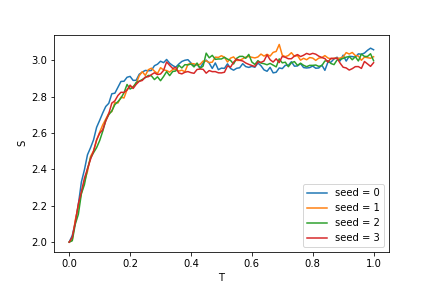
\includegraphics[scale=.6]{随机微分方程解2的多条轨道S-T.png}
    \caption{随机微分方程2解的多条轨道S-T}
    \label{fig:SDE2_S}
    \end{figure}


我们看到$S_t$和$X_t$的曲线是十分相似的,所以我们初步推断$S_t$是受$X_t$影响,不断趋向$X_t$,最终区域稳态$v$。


\begin{figure}[H]
    \centering
    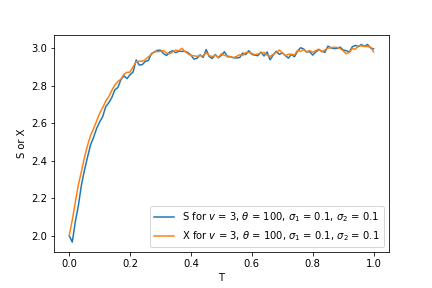
\includegraphics[scale=.6]{随机微分方程解2的多条轨道SX-T.png}
    \caption{随机微分方程2解的多条轨道S, X-T}
    \label{fig:SDE2_SX}
    \end{figure}


我们画出了价格与价值比值曲线随时间$T$的变化,可以看到他很快就趋于1,然后受噪声和随机性的影响不断振荡。

\begin{figure}[H]
    \centering
    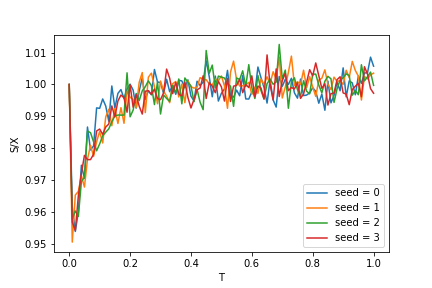
\includegraphics[scale=.6]{随机微分方程解2的多条轨道Ratio-T.png}
    \caption{随机微分方程2解的多条轨道S/X-T}
    \label{fig:SDE2_Ratio}
    \end{figure}


接下来我们实验观察参数对轨道的影响。我们的所有实验都是在控制变量的条件下进行的,被控制的变量默认为$\alpha=1, v=3, \sigma=0.1, \theta=100, \sigma_1 = \sigma_2 = 0.1, x_0=s_0=2$。同样地,$d_t = 0.01$,一共取100个个点,区间是$[0, 1]$。


\begin{figure}[H]
    \centering
    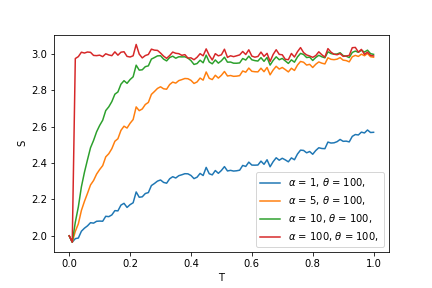
\includegraphics[scale=.6]{随机微分方程解2参数alpha.png}
    \caption{参数 $\alpha$ 对随机微分方程2解的轨道影响}
    \label{fig:SDE12_alpha}
    \end{figure}

首先,$\alpha$ 以与图\ref{fig:SDE1_alpha}相似的方式,通过影响价值曲线$X_t$的方式影响$S_t$。$\alpha$决定了两者向稳态的收敛速率。


\begin{figure}[H]
    \centering
    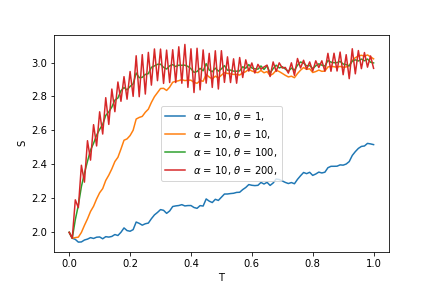
\includegraphics[scale=.6]{随机微分方程解2参数theta.png}
    \caption{参数 $\theta$ 对随机微分方程2解的轨道影响}
    \label{fig:SDE2_theta}
    \end{figure}

$\theta$ 同样决定了价格曲线$S_t$收敛的速率,当$\theta$过小的时候收敛很慢,但是当$\theta$过大的时候就会发生振荡,这是因为将$S_t$向$X_t$修正的时候,修正过大。


\begin{figure}[H]
    \centering
    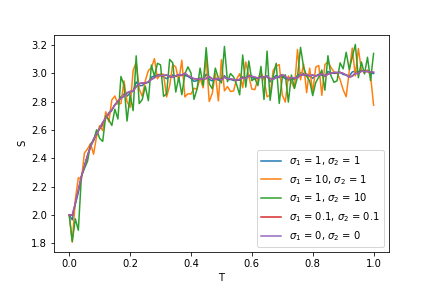
\includegraphics[scale=.6]{随机微分方程解2参数sigma.png}
    \caption{参数 $\sigma$, $\sigma_1$ 和 $\sigma_2$ 对随机微分方程2解的轨道影响}
    \label{fig:SDE2_sigma}
    \end{figure}    


$\sigma_1$ 和 $\sigma_2$ 同样还是影响正态分布噪音的方差


\begin{figure}[H]
    \centering
    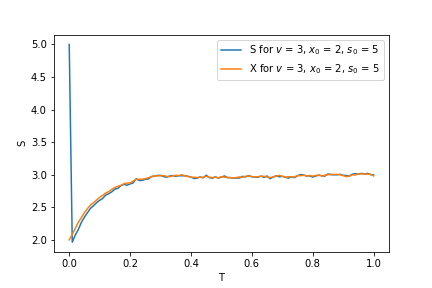
\includegraphics[scale=.6]{随机微分方程解2参数初值.png}
    \caption{参数 $v$ 和初值对随机微分方程2解的轨道影响}
    \label{fig:SDE2_x0}
    \end{figure}

$v$ 代表了$S_t$ 和 $X_t$ 最终的稳态,而$x_0$和$s_0$表示两条曲线的初值,我们可以发现$S_t$很快向$X_t$收敛,这里是因为$\alpha\theta dt = 1$的原因。


\begin{table}[H]
    \centering
    \caption{不同参数下的 $E(S_1)$ 和 $D(S_1)$}
    \begin{tabular}{l|l|l|l|l|l}
    \hline
    $\alpha$                           & $E(S_1)$  & $D(S_1)$  & $\theta$               & $E(S_1)$  & $D(S_1)$  \\ \hline
    1                               & 2.636873 & 0.004301 & 1                   & 3.000939 & 0.000513 \\ 
    5                               & 2.99551  & 0.000966 & 10                  & 3.000939 & 0.000513 \\ 
    10                              & 3.000939 & 0.000513 & 100                 & 3.000939 & 0.000513 \\ 
    100                             & 2.999987 & 0.000101 & 1000000                 & 3.000939 & 0.000513 \\ \hline
    $\sigma,\ \sigma_1,\ \sigma_2$ & $E(S_1)$  & $D(S_1)$  & $v, x_0, s_0$ & $E(S_1)$  & $D(S_1)$  \\ \hline
    0.1, 0.1, 0.1                   & 3.000939 & 0.000513 & 3, 2, 2       & 3.000939 & 0.000513 \\ 
    0.1, 100, 0.1                 & 3.000939 & 0.000513 & 5, 2, 2       & 5.000885 & 0.000513 \\ 
    0.1, 0.1, 100                  & 3.000939 & 0.000513 & 3, 7, 2       & 3.004932 & 0.000513 \\ 
    1, 0.1, 0.1                  & 3.009625 & 0.05126  & 3, 2, 7       & 3.004799 & 0.000513 \\ \hline
    \end{tabular}
    \end{table}

我们看到$\alpha$与$D(S_1)$相关,$\theta$与期望和方差都不相关,$\sigma$的平方与$D(S_1)$成正比,$\sigma_1$与$\sigma_2$与$D(S_1)$成正比,$v$在理想情况下等于$E(S_1)$,$x_0$与$s_0$没有直接关系,但是是在能够在迭代步数内收敛的情况下。






\section{总结与感悟}
这次大作业对我来讲是一次全新的体验。首先我学习到了如何通过数值解法解随机微分方程,这对我的python代码能力是一个很大的提升。同时数值解法的学习也让我对随机过程的理论有更深的理解,数值解法与理论解法是两种不同的角度,但是殊途同归,都会引导出我们对微分方程的解的理解。另外这个随机微分方程的主题也十分有趣,我虽然对金融经济一无所知,但是方程的金融意义让我对随机过程也有了更深刻的认识。最后十分感谢熊老师这学期的辛勤付出,不仅是课程上的辛勤教导,更感谢熊老师在疫情期间为同学们送饭帮助我们的辛勤付出,老师的行动对我的学术和人生都是很大的鼓舞!

最后感谢老师和助教这一学期的辛勤付出,让我们的这门课即使在疫情期间也有这样良好的效果!感谢大家的付出!






% \bibliographystyle{plain}
% \bibliography{references}
\end{document}